% Generated by the Rust camera-count study.
\section{Camera-count and baseline audit}
The current sampler was evaluated on 64 consecutive matched rooms (seeds 0--63), 1--12 cameras and baseline values 0, 0.5 and 1 at aspect ratio 1.60. Geometry, people and appearance were unchanged between requests; complete camera sets were resampled, so different counts are not necessarily nested prefixes. 0 of 2304 requested sets were rejected by the bounded sampler; all failures remain in the downloadable report. Camera-center and optical-axis measurements use 33 synchronized path samples. Reference-edge overlap uses the production 13$\times$9 first-surface proxy at five times, rather than rendered pixels.

At one camera the baseline imposes no pair constraint. The serialized controls and per-count mixed-rig/coherence diagnostics accompany every requested set. Nominal advanced controls describe proposals; admission also accounts for calibrated lens footprints and room clearance. Group covariance spread constrains overall anisotropy, not every nearest neighbor. Visible-region target variation samples reference-visible surface patches and ranks feasible candidates for count-aware nearest-peer spacing, optical-axis separation and additional primary-room proxy surface cells. The soft distance scale is room diagonal divided by the square root of camera count. Temporal paths can remain related deformations of an existing route; varied gaze is not independent route topology. There is no explicit 90-degree optical-angle cap.

\begin{table}[htbp]\centering\small
\begin{tabular}{rrrrrr}\toprule
$b$ & Cameras & Accepted & NN (m) & Max angle ($^\circ$) & Targets (m) \\
\midrule
0.0 & 2 & 64/64 & 0.18 & 1.3 & 0.03 \\
0.0 & 4 & 64/64 & 0.15 & 4.2 & 0.05 \\
0.0 & 8 & 64/64 & 0.11 & 6.2 & 0.06 \\
0.0 & 12 & 64/64 & 0.09 & 6.9 & 0.06 \\
0.5 & 2 & 64/64 & 2.09 & 27.2 & 0.33 \\
0.5 & 4 & 64/64 & 1.43 & 45.6 & 1.63 \\
0.5 & 8 & 64/64 & 1.05 & 76.3 & 2.25 \\
0.5 & 12 & 64/64 & 0.85 & 97.7 & 2.79 \\
1.0 & 2 & 64/64 & 4.32 & 71.9 & 1.87 \\
1.0 & 4 & 64/64 & 2.69 & 144.7 & 4.94 \\
1.0 & 8 & 64/64 & 1.41 & 156.0 & 5.73 \\
1.0 & 12 & 64/64 & 1.19 & 166.6 & 6.42 \\
\bottomrule\end{tabular}
\caption{Current matched placement audit. NN is the pooled camera-level initial nearest-neighbor median; angle and target diameter are room-level medians. Failed sets have no placement measurements. These denominators differ from rendered pixel overlap.}\label{tab:camera-counts}
\end{table}

Similar absolute trajectories have RMS center separation below 0.15 m and RMS optical-axis difference below $5^\circ$. Shape similarity instead removes each start position and normalizes the RMS displacement residual by the larger RMS travel, with a diagnostic threshold of 0.25; static pairs are excluded. Close stereo views can intentionally satisfy the pose threshold. A common-axis least-squares residual measures convergence of initial optical-axis lines; parallel or ill-conditioned lines have no reported focus. Neither statistic proves perceptual repetition or reconstruction utility.

\begin{figure}[p]\centering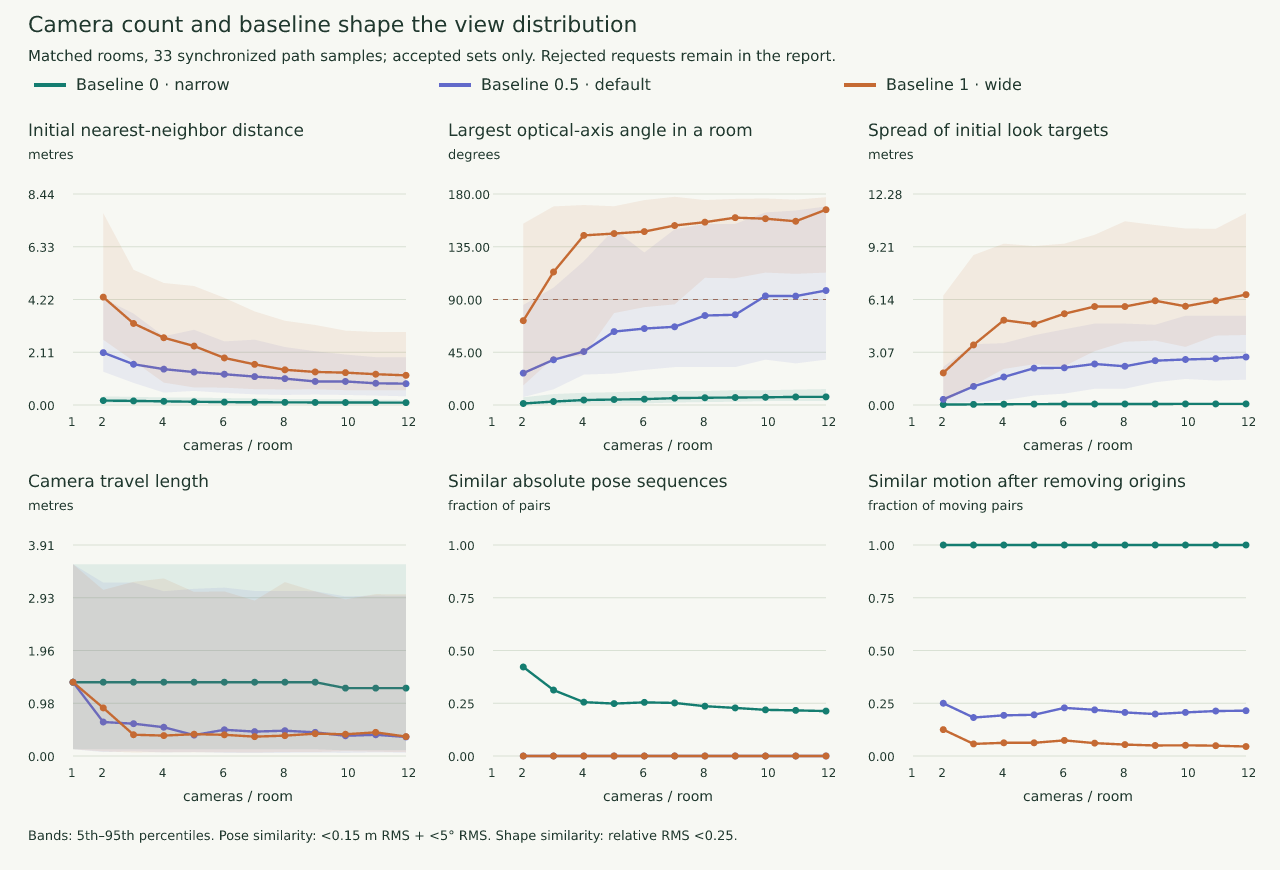
\includegraphics[width=\linewidth]{generated/camera_count_statistics.png}
\caption{Camera-count distributions at three baseline settings. Room-level viewing-angle/target statistics and camera-level spacing use their own denominators. Repeated path shapes are measured separately from repeated absolute poses.}\label{fig:camera-count-statistics}\end{figure}
\begin{figure}[p]\centering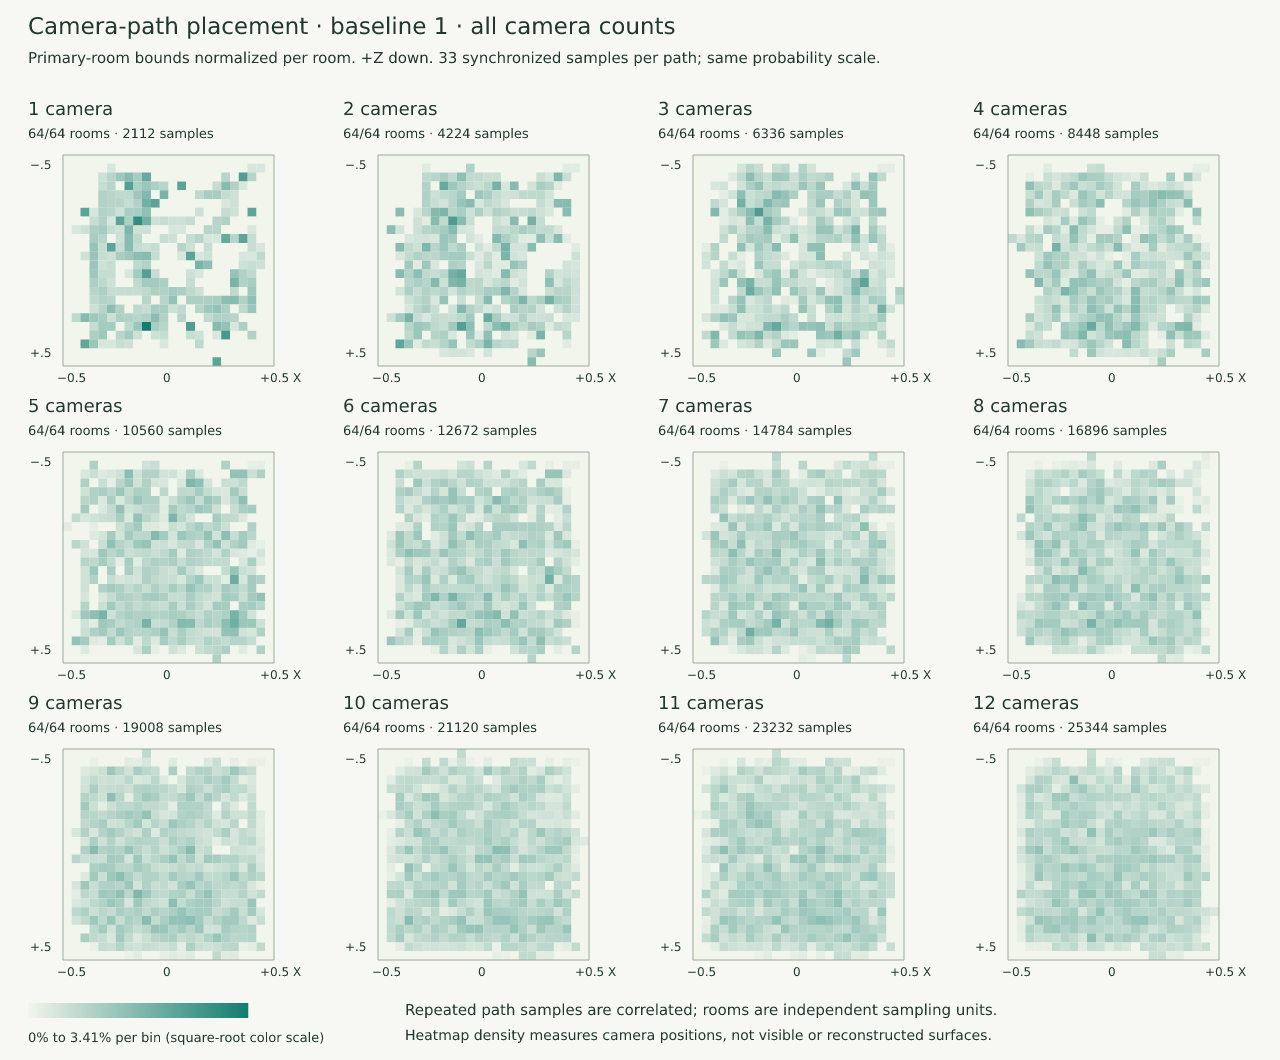
\includegraphics[width=\linewidth]{generated/camera_count_heatmap.png}
\caption{Baseline 1 camera-path heatmaps for 1--12 views: 33 synchronized samples per camera, primary-room bounds normalized per room and +Z down. A common probability color scale is used. These show positions, not reconstructed-surface coverage.}\label{fig:camera-count-heatmap}\end{figure}
\begin{figure}[p]\centering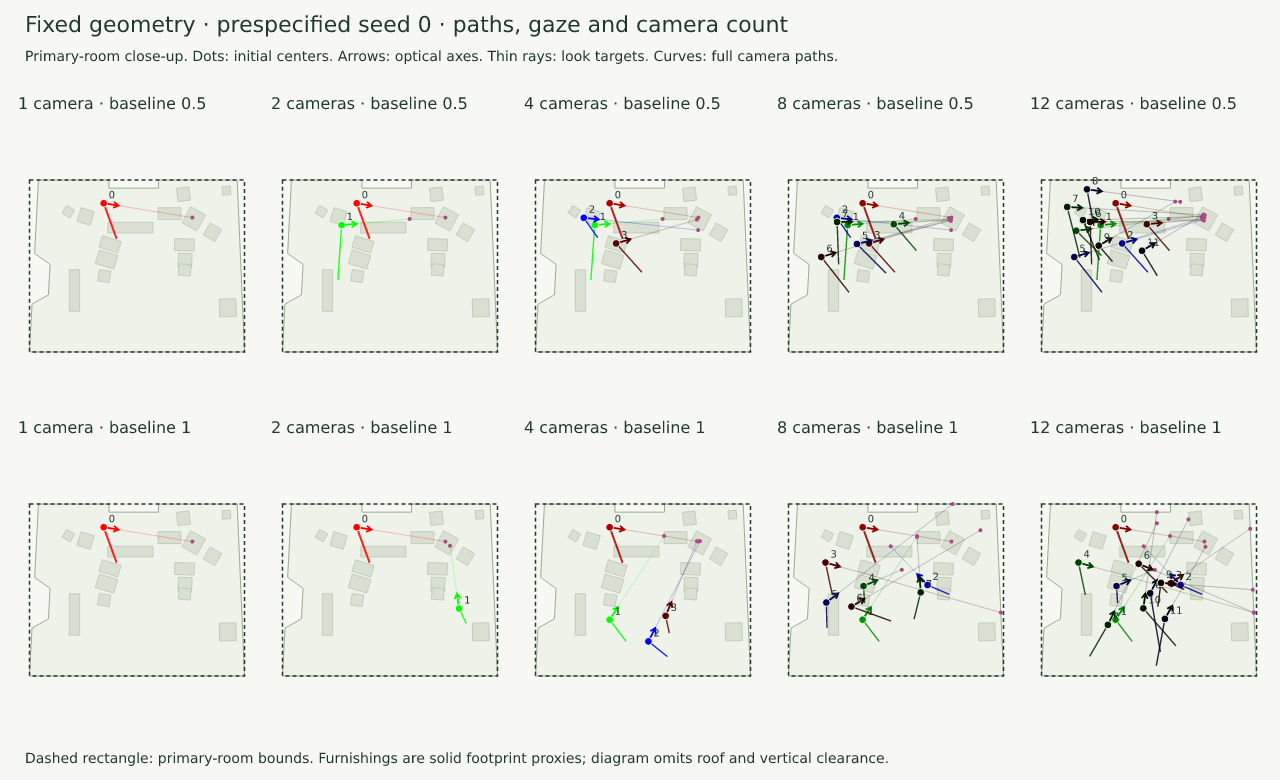
\includegraphics[width=\linewidth]{generated/camera_count_schematics.png}
\caption{Prespecified first room, fixed geometry and people, default/wide baselines and increasing camera counts. Full paths, initial optical directions and look targets expose the shared-content proposal. Rejected requests are retained.}\label{fig:camera-count-schematics}\end{figure}

\clearpage

\subsection{Native rendered overlap across camera counts}
The rendered check uses 2 prespecified matched room families, 12 configurations and 312 camera/time views: counts 2, 4, 8 and 12 at all three baselines and both trajectory endpoints, with 320$\times$200 images, static human density 0.25 and native shadows, material synthesis and diffuse GI retained. The executable and every channel are hash-bound. Rendered centers and optical axes match the CPU audit within $10^{-4}$ m and $10^{-5}$ per direction component. Table~\ref{tab:camera-count-rendered} separates mean directed pair overlap from mean source-view visibility in any peer, and reports the smallest reference-edge overlap over the sampled rooms/times. These do not measure unique scene-surface coverage.

\begin{table}[htbp]\centering\small
\begin{tabular}{rrrrrr}\toprule
$b$ & Cameras & Pair (\%) & Any peer (\%) & Min ref. (\%) & Components \\
\midrule
0.0 & 2 & 84.0 & 84.0 & 75.4 & 1 \\
0.0 & 4 & 82.3 & 93.0 & 62.3 & 1 \\
0.0 & 8 & 81.1 & 96.9 & 62.3 & 1 \\
0.0 & 12 & 80.6 & 98.3 & 59.3 & 1 \\
0.5 & 2 & 58.3 & 58.3 & 32.6 & 1 \\
0.5 & 4 & 52.7 & 76.9 & 32.6 & 1 \\
0.5 & 8 & 54.9 & 91.4 & 32.6 & 1 \\
0.5 & 12 & 53.6 & 93.7 & 32.6 & 1 \\
1.0 & 2 & 39.7 & 39.7 & 29.7 & 1 \\
1.0 & 4 & 46.2 & 74.5 & 26.2 & 1 \\
1.0 & 8 & 39.5 & 86.1 & 14.7 & 1 \\
1.0 & 12 & 39.3 & 90.8 & 14.7 & 1 \\
\bottomrule\end{tabular}
\caption{Native first-surface co-visibility; glass follows the solid annotation convention. Components is the largest number of connected components when an undirected edge requires at least 5\% shared pixels in both directions. Room families are the independent units; camera pairs and endpoints are correlated.}\label{tab:camera-count-rendered}\end{table}
\begin{figure}[htbp]\centering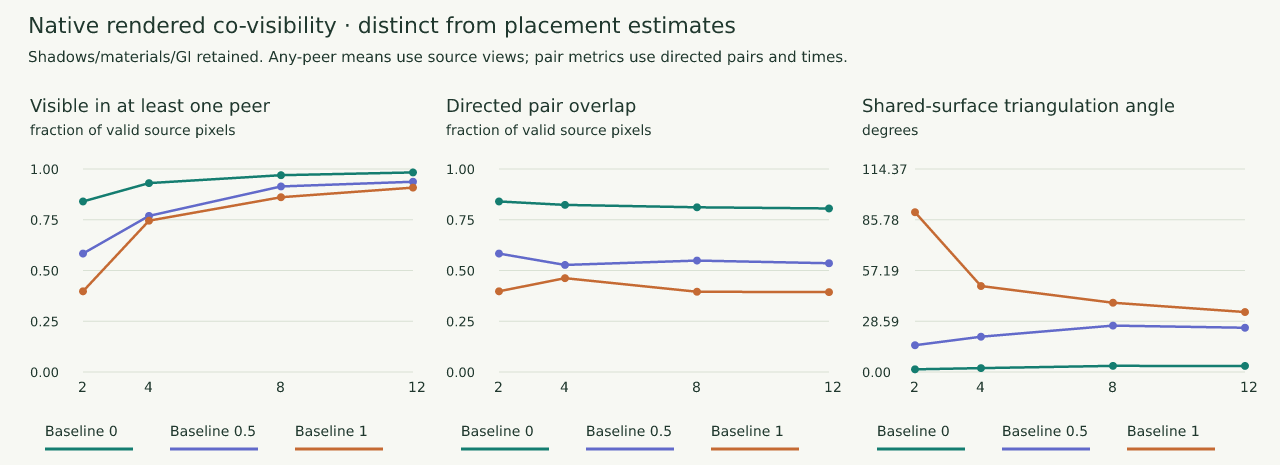
\includegraphics[width=\linewidth]{generated/camera_count_rendered.png}
\caption{Measured native visibility and triangulation at increasing camera counts. Any-peer visibility is averaged over source views, other means over directed pairs. More peer views increase any-peer visibility without proving broader unique surface coverage.}\label{fig:camera-count-rendered}\end{figure}

\subsection{Visual effect of camera baseline}
Each column resamples a complete four-camera group over identical geometry, people, materials and lighting. Camera indices identify group members, rather than fixed physical viewpoints across columns. These are the first two prespecified native families, with every view retained at t=0 and no per-image exposure correction. They contribute no extra rooms to the population denominator.

\begin{figure}[p]\centering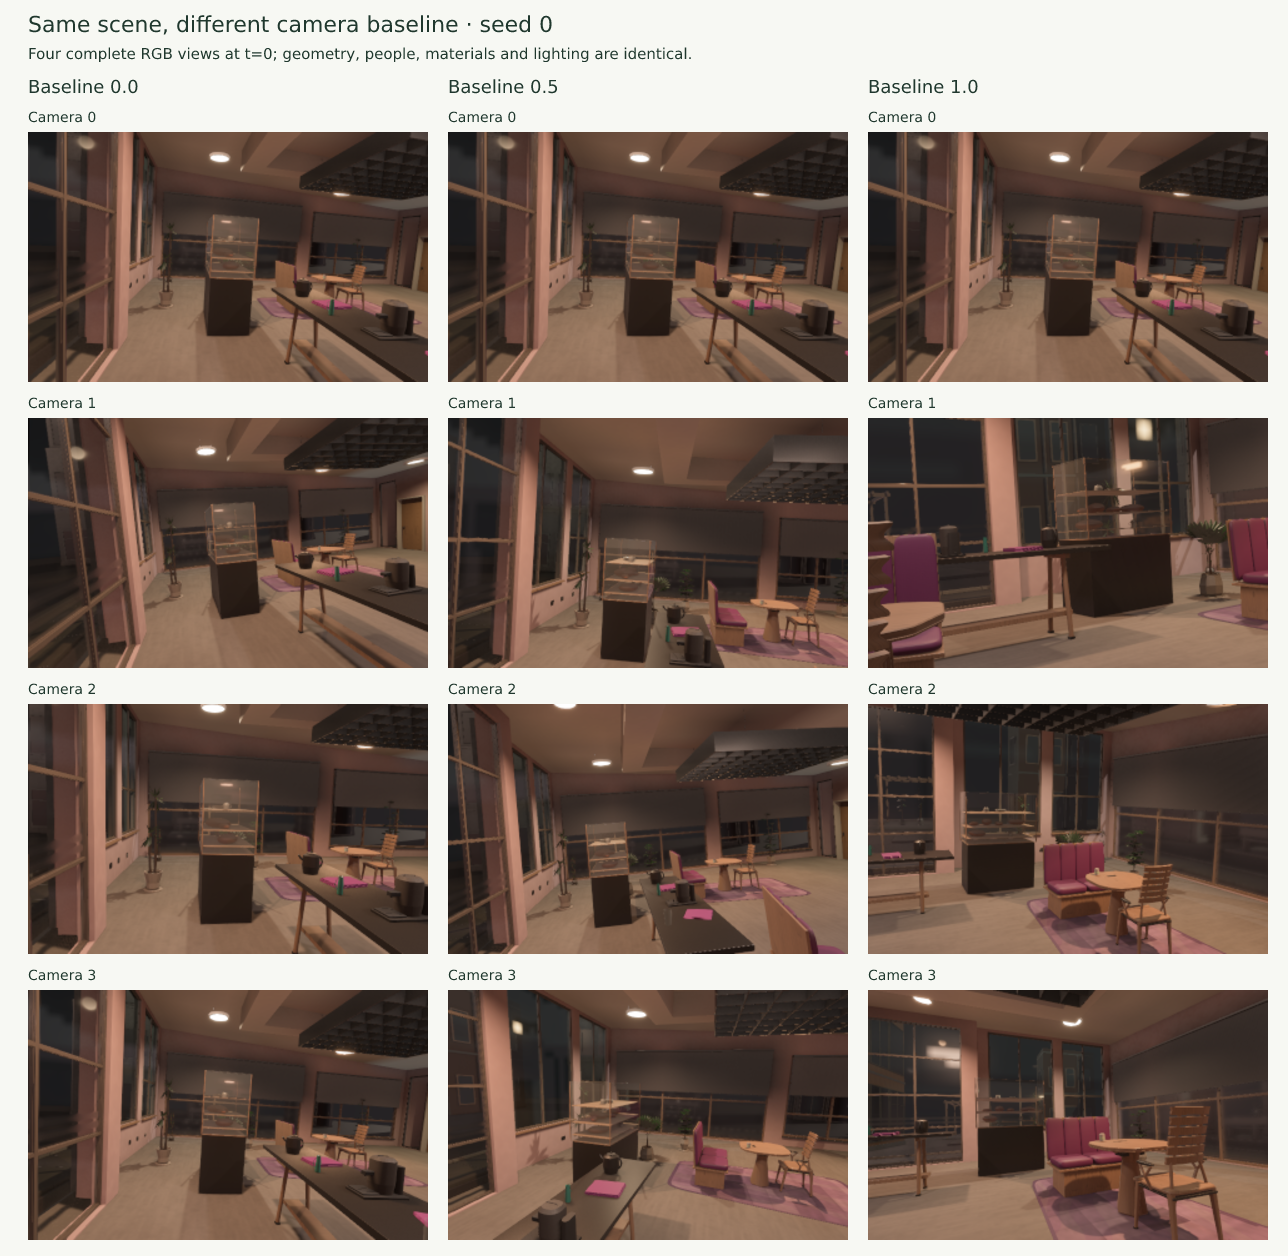
\includegraphics[width=\linewidth,height=.82\textheight,keepaspectratio]{generated/camera_count_baseline_s0.png}
\caption{Fixed room 0: narrow, default and wide baseline settings (0, 0.5 and 1) from left to right. Rows retain all four native RGB views at 320$\times$200. Perspective and shared content change with the camera policy; scene content is invariant.}\label{fig:camera-baseline-0}\end{figure}

\begin{figure}[p]\centering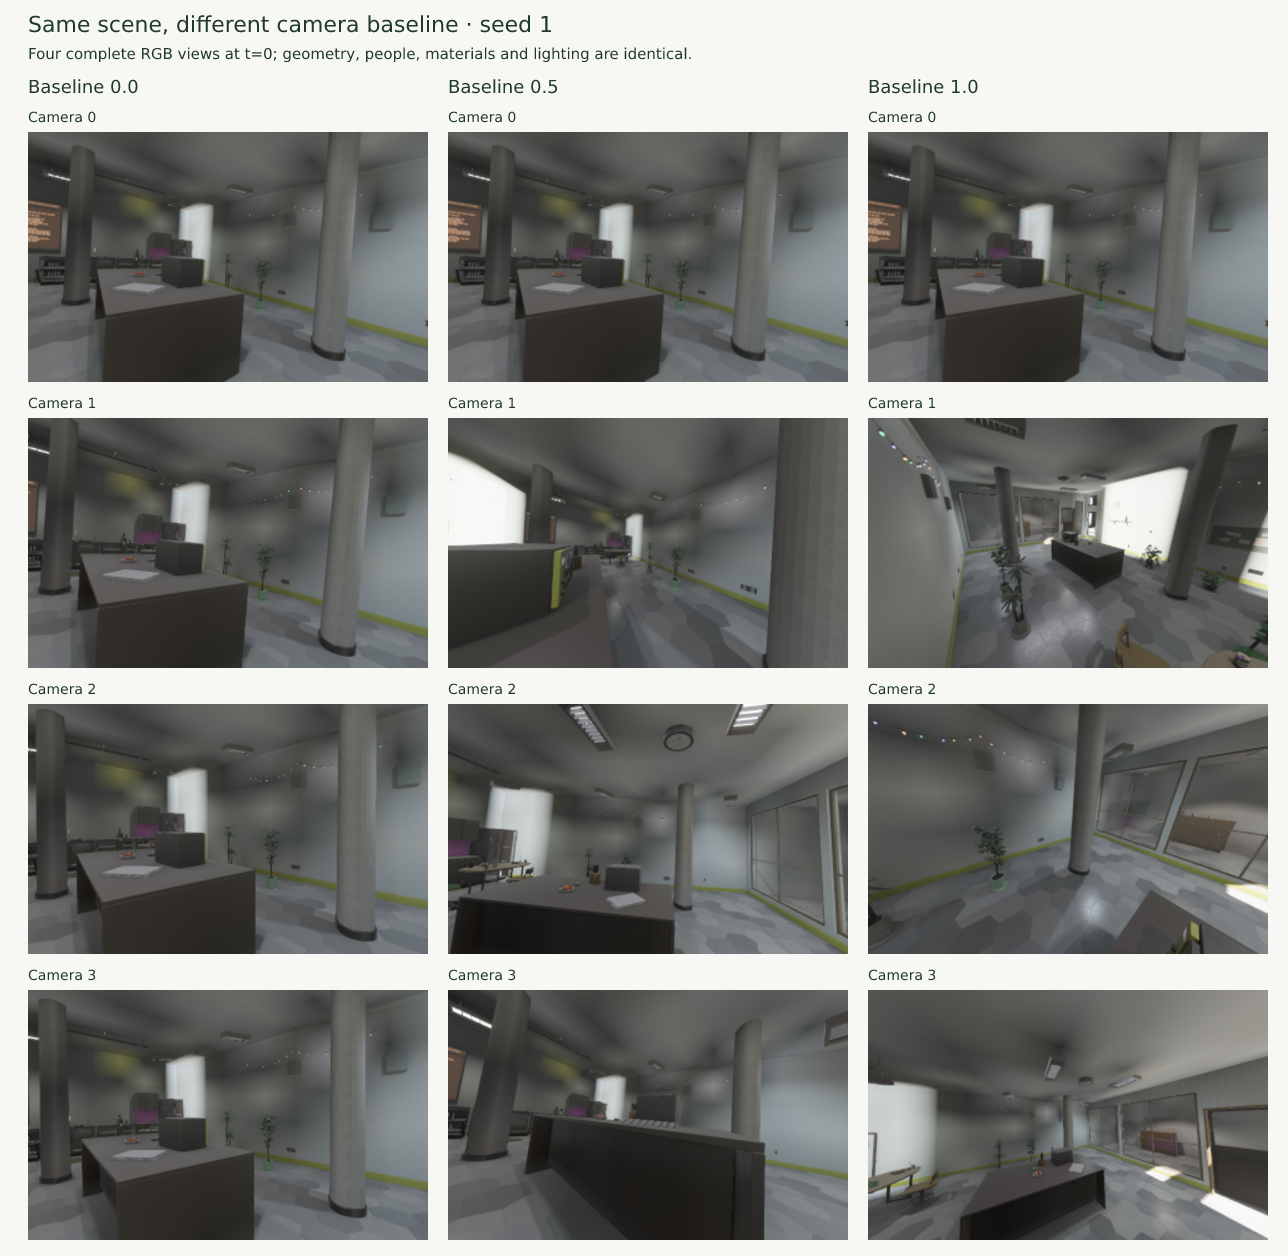
\includegraphics[width=\linewidth,height=.82\textheight,keepaspectratio]{generated/camera_count_baseline_s1.png}
\caption{Fixed room 1: narrow, default and wide baseline settings (0, 0.5 and 1) from left to right. Rows retain all four native RGB views at 320$\times$200. Perspective and shared content change with the camera policy; scene content is invariant.}\label{fig:camera-baseline-1}\end{figure}

\clearpage
